%
% File acl2019.tex
%
%% Based on the style files for ACL 2018, NAACL 2018/19, which were
%% Based on the style files for ACL-2015, with some improvements
%%  taken from the NAACL-2016 style
%% Based on the style files for ACL-2014, which were, in turn,
%% based on ACL-2013, ACL-2012, ACL-2011, ACL-2010, ACL-IJCNLP-2009,
%% EACL-2009, IJCNLP-2008...
%% Based on the style files for EACL 2006 by 
%%e.agirre@ehu.es or Sergi.Balari@uab.es
%% and that of ACL 08 by Joakim Nivre and Noah Smith

\documentclass[11pt,a4paper]{article}
\usepackage[hyperref]{acl2019}
\usepackage{times}
\usepackage{latexsym}
\usepackage{hyperref}
\usepackage{algpseudocode}
\usepackage{algorithm}
\algnewcommand\algorithmicforeach{\textbf{for each}}
\algdef{S}[FOR]{ForEach}[1]{\algorithmicforeach\ #1\ \algorithmicdo}
\usepackage{graphicx}
\usepackage[caption=false]{subfig}

% \aclfinalcopy % Uncomment this line for the final submission
%\def\aclpaperid{***} %  Enter the acl Paper ID here

%\setlength\titlebox{5cm}
% You can expand the titlebox if you need extra space
% to show all the authors. Please do not make the titlebox
% smaller than 5cm (the original size); we will check this
% in the camera-ready version and ask you to change it back.

\newcommand\BibTeX{B\textsc{ib}\TeX}

\title{Comparative study of Dask and Spark for neuroimaging pipelines}

\author{Mathieu Dugr{\'e} \\
  Concordia University \\
  \texttt{mathieu.dugre@mail.concordia.ca}\\}

\date{}

\begin{document}
\maketitle
\begin{abstract}

% Topic
As the amount of data increases and is easier to access, Big Data processing becomes
critical in neuroimaging.
% Problem
This is an issue as the currently used frameworks are specialized for neuroimaging
and not Big Data concerns. This can lead to performance decrease or limit the
research we can perform.
% Relevance
The usage of Big Data framework is beneficial to this problem. The state-of-the-art
general purpose Big Data framework Spark has its code base written in Scala, while
our laboratory mostly uses Python. This can be problematic since it is harder to port
our pipelines to the framework. Also, theoretically, it leads to performance
decrease.

% Approach
We propose to use Dask since it provides native Python parallelism to pipelines while
providing support to familiar API from the Python's scientific ecosystem. However
there are few comparisons of Spark and Dask; especially in neuroimaging. Moreover,
these studies were done when Dask was still an immature framework which make those
study unfair nowadays. This is our motivation to compare the latest version of Dask
with Spark.
% Methods (one sentence)
To evaluate the frameworks, we focus on their performance and their scheduler.

% Key Impact
Our study demonstrates the potential of using Dask as the framework to build
neuroimaging pipelines.

\end{abstract}

\section{Introduction}
% Context
With the increasing number of data available in neuroimaging \citep{ALFAROALMAGRO:18,
UKBioBank:18} the processing of Big Data becomes critical. Frameworks like Nipype
\citep{Nipype:11} are usually used to create neuroimaging pipelines however it is
worth considering the use of general purpose Big Data frameworks
\citep{Hayot-Sasson:17}. In that research, Spark \citep{Spark:16} was a natural
choice as it is the state-of-the-art framework for Big Data. However, as our
laboratory works mostly with Python, we want to know if Dask \citep{Dask:15}, a
Python written framework, could bring better or similar performances while
facilitating usage.

%Similarities
Spark and Dask offer in-memory computing, data locality and lazy evaluation; which is
common for Big Data framework. Both their scheduler operate dynamically. This is good
when the runtimes are not known ahead of time \citep{Dask:15}. Over these
similarities, the frameworks are quite different.

% Spark
On the one hand, we have Spark which provides a high-level API. This allows the
scheduler to perform more optimizations which makes it well suited for neuroimaging
analysis that often require the usage of pipeline with multiple steps. However,
Spark's code base is in Scala which theoretically can lead to slow down in execution
due to a required serialization. Moreover, while Spark's API is flexible and allows
most implementations, it differs from the ones seen in the Python's ecosystem.

% Dask
On the other hand, Dask was created with the purpose to natively parallelize Python
pipelines while keeping the syntax of familiar API from the Python's scientific
ecosystem. However, Dask is still a young framework with work to be done; it's API
does not completely replicate the library it supports. While its lower-level API
allows the implementation of more complex algorithms it sacrifice a layer of
optimization.
% Related work
Previous work by \citet{Mehta:17} shows that Dask had significant overhead and was
hard to debug.
% What issues your work addresses
Dask was immature at the time and a lot of change was brought to the framework.
Therefore we think it is valuable to re-compare it with Spark.

%% Dask API
The Dask API we decide to use for our comparison are Dask bag, delayed and futures.
Dask bag offer an easy API to parallelize data. Dask delayed offer a lower-level API
that offer more flexibility; this is good to implement more complex task that do not
fit in the Dask bag framework. Dask futures is a real time API. Both Dask bag and
delayed apply lazy evaluation to tasks while futures trigger them directly.

% Methods used (summary)
The project aims to compare the state-of-the-art general purpose framework Spark with
the newcomer Dask. We decide to compare the performance of Spark and Dask on a custom
incrementation pipeline to simplify the effect of the algorithm on the comparison.
Then we assess the frameworks on two real-life applications: (1) histogram of the
voxels intensity in a 3d images (2) BIDS example.

% Implications of our research
The result from our project help in deciding if Dask is a good choice to build
neuroimaging pipelines.


%%%%% MATERIAL AND METHODS %%%%%%
\section{Material and Methods}
%% Material
We compare Dask(\textbf{v1.1.4}) and Spark(\textbf{v2.4.0}) based on two metrics
their scheduling and their makespan performance. All scripts used to perform our
experiments are available at
\href{https://github.com/mathdugre/paper-big-data-engines}{https://github.com/mathdugre/paper-big-data-engines}.
For our experiments we used Compute Canada Cloud where each instance has 8 cores,
30GB RAM, 10GB bandwidht and is dedicated.
 
%% Incrementation
\subsection{Incrementation} As our first experiment to benchmark the frameworks we
used a simple incrementation pipeline (see Algorithm \ref{alg:incrementation}). It
loads chunks from the 75GB BigBrain\citep{ds052:01} image, increment its value by 1 a
determined number of time and save the result to an nfs as a Nifti image.
Incrementting the data reduce the caching effect. This experiment allows us to study
the behaviour of the frameworks when all input are processed independently; i.e. each
task in the graph only depend on the previous one (see \ref{Figure fig:tg-inc}).

This experiment refers to the implementation of the Spark pipelines purposed in
\citet{Hayot-Sasson:17}.

\begin{algorithm}\caption{Incrementation}\label{alg:incrementation}
    \begin{algorithmic}
    \Require $x$, a sleep delay in float
    \Require $file$, a file containing a chunk
    \Require $fs$, nfs to save image to.
    \State read $chunk$ from $file$
    \ForEach{$i \in iterations$}
    \ForEach{$chunk \in image$}
        \State $chunk\gets chunk+1$
        \State sleep $x$
    \EndFor
    \EndFor
    \State save $chunk$ to $fs$
\end{algorithmic}
\end{algorithm}

\begin{figure}[ht]
    \centering
    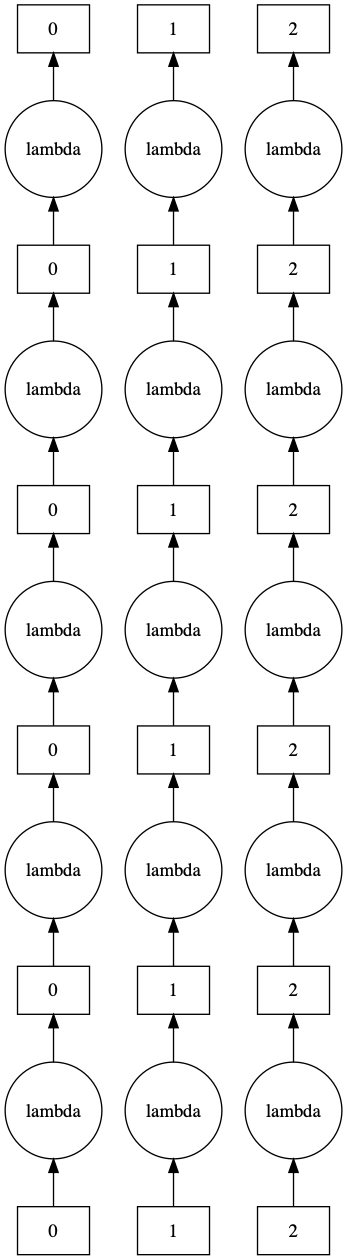
\includegraphics[width=0.125\textwidth, angle=-90]{images/incrementation-task-graph.png}
    \caption{Task graph for Incrementation}
    \label{fig:tg-inc}
\end{figure}

% Histogram
\subsection{Histogram}
For our second experiment we find the frequency of the voxels intensity in BigBrain
and save them as a tuple in a file. In this experiment the end results depends on all
of the input results (see \ref{Figure fig:tg-histo}). This allows us to study the behaviour
of the framework when task are dependent. Also this application require data
shuffling thus inter worker communication. In this application we decided to omit the
dask futures api as it is less realistic for this use case.

\begin{figure}[ht]
    \centering
    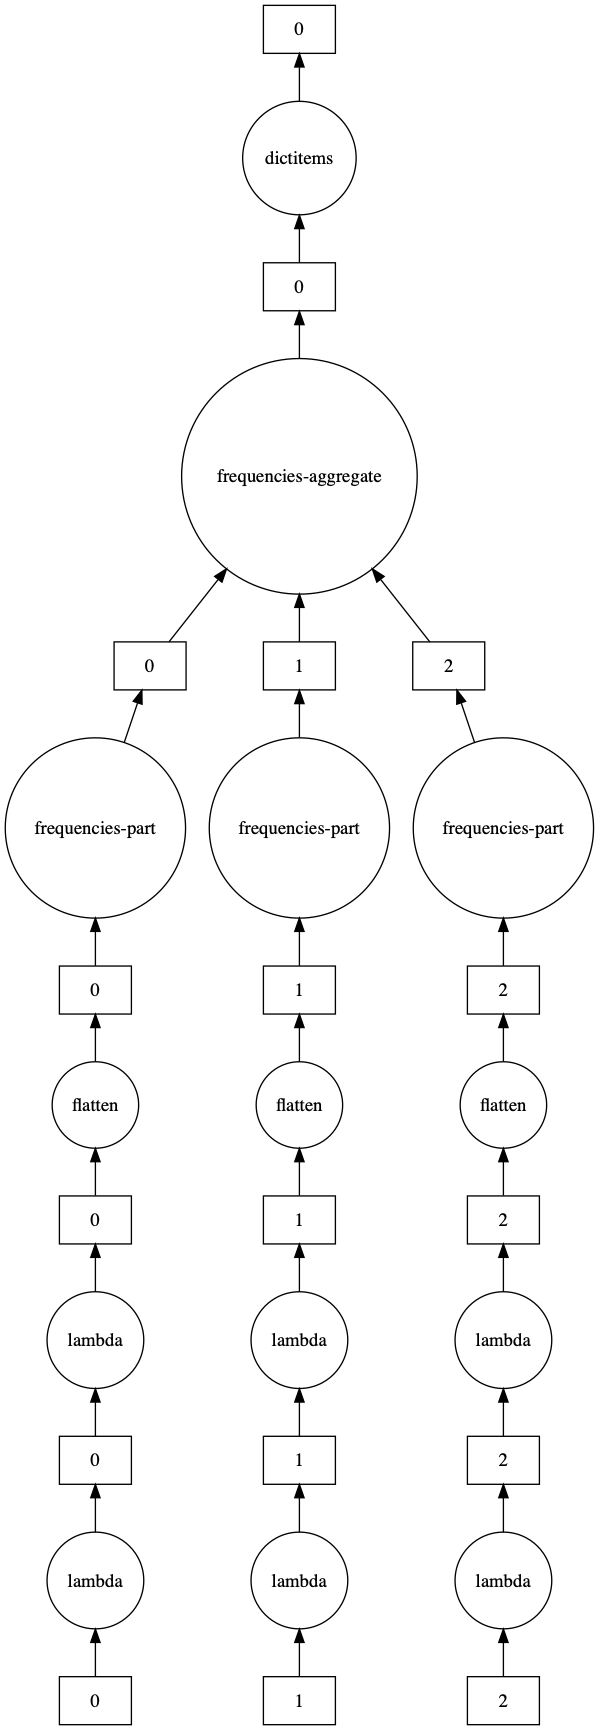
\includegraphics[width=0.16\textwidth, angle=-90]{images/histogram-task-graph.png}
    \caption{Task graph for Histogram}
    \label{fig:tg-histo}
\end{figure}

% BIDS Example
\subsection{BIDS Example}
Our last experiment compare both frameworks on the BIDS Example algorithm.
% Specify more details and the data set used
% SECTION TO COMPLETE -- Experience not done yet


%% Performance
\subsection{Experiments}
Our experiments have for goal to see how the frameworks react to different
environments and tasks types.

%% Incrementation
For the incrementation experiment, we
%% Node
first vary the number of instances in our cluster environment. We test with 1, 2, 4,
and 8 instances. From this we can evaluate the level of parallelism offered by
both framework.

%% Iterations
Secondly, we modify the number of iterations we perform on the increment task between
the experiment. We use 1, 10 and 100 iterations. This allow the study of the
schedulers different amount of task are to be performed.

%% Sleep delay
Thirdly, we change the sleep delay in the increment tasks. We fix a 1, 4 and 16 and
64 seconds sleep time for each iterations. This allow us to test the effect of tasks
with different time length.

%% Splits
Finally, we seperate the BigBrain in different number of splits. We seperate it in
30, 125 and 750 splits; around 2.5GB, 0.6GB and 0.1GB, respectively. From that we can
evaluate the framework with task of different size and IO requirements.

%% Baseline
Our baseline for all experiment is 10 iterations, 4 sleep delay, 125 splits running
on 8 instances.

%% Histogram
For the histogram experiment, we vary the number of instances, as above. We also
change the number of splits as above.

%% BIDS Example
For the BIDS example experiment, we vary the number of instances, again as above.

% Note
Note that the code implemented might not be optimal. However we hope to provide a
baseline assessment of Dask and Spark.


%%%%% RESULTS %%%%%
\section{Results}

%%% INCREMENTATION %%%
%% Instances
\subsection{Experiment 1: Number of instances}
Figure \ref{fig:inc_worker}(a) shows that the incease in performance is not
proportional to the number of worker which differ form what we would expect; it even
decrease when we reach 8 workers. This is explained by an increase in IO overhead
corrolated to the number of workers (Figure \ref{fig:inc_worker}(b)), as more worker
access the nfs simultaneously it increase the stress put on the system which result
in bottleneck, errors and slow down.

On the one hand, Dask seems better when using a single worker. On the other hand,
Spark makespan decrease faster for higher level of parallelism. However Dask is
constently faster then spark which make us think it has a better scheduler.

\begin{figure}[htp]
    \centering
    \subfloat[Incrementation makespan]{%
      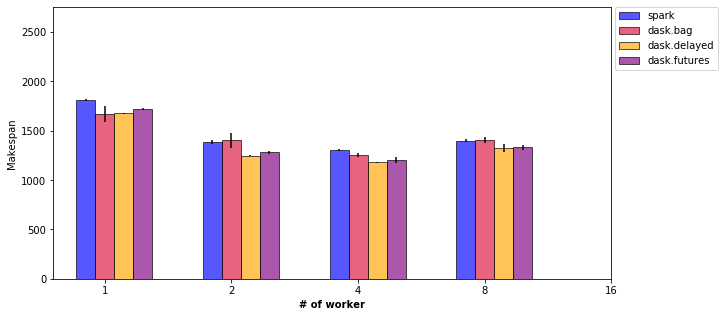
\includegraphics[clip,width=\columnwidth]{images/inc_worker.png}%
    }
    
    \subfloat[Incrementation total time]{%
      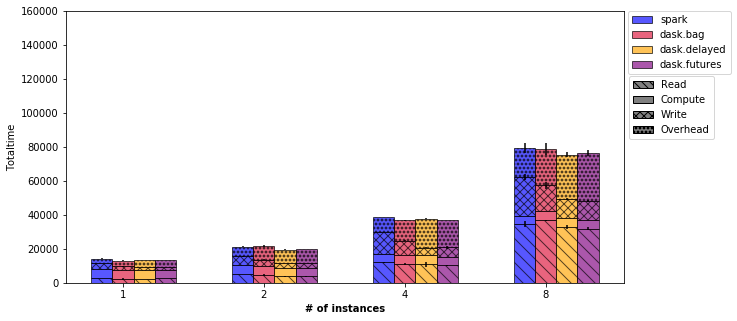
\includegraphics[clip,width=\columnwidth]{images/inc_idle_worker.png}%
    }
    \caption{125 splits, 10 iterations, 4 sec. sleep delay}
    \label{fig:inc_worker}
\end{figure}



%% Iterations
\subsection{Experiment 1: Number of iterations}
In Figure \ref{fig:inc_itr} we see that spark and the dask bag api are equivalent in
term of performance. The dask delayed api seems to perform well with low amount of
task but grow faster the spark and dask bag. We think this is because dask delayed
often schedule a block on different thread of the same worker which cause small delay
everytime due to inter thread data communication. This is good when there is fewer
tasks as is make the IO between block go out of sync hence lowering the IO bottleneck
however as the number of tasks increases those small delays become significant. The
dask futures api seems to outperform all the other apis but this is most likely
because the tasks are not inter dependent thus this application benifits from the
less optimal but faster scheduling brought by dask futures.

\begin{figure}[htp]
    \centering
    \subfloat[Incrementation makespan]{%
      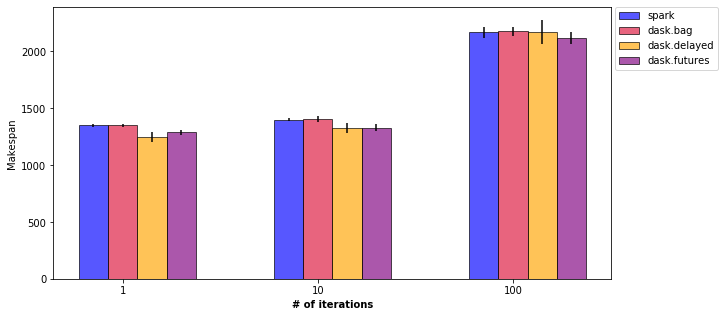
\includegraphics[clip,width=\columnwidth]{images/inc_itr.png}%
    }
    
    \subfloat[Incrementation total time]{%
      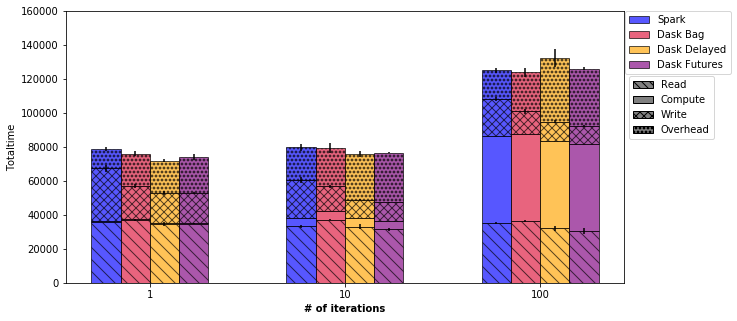
\includegraphics[clip,width=\columnwidth]{images/inc_idle_itr.png}%
    }
    \caption{125 splits, 4 sec. sleep delay, 8 instances}
    \label{fig:inc_itr}
\end{figure}


%% Sleep time
\subsection{Experiment 1: Sleep delay}
As Figure \ref{fig:inc_sleep} 
% Not sure what to conclude.

\begin{figure}[htp]
    \centering
    \subfloat[Incrementation makespan]{%
      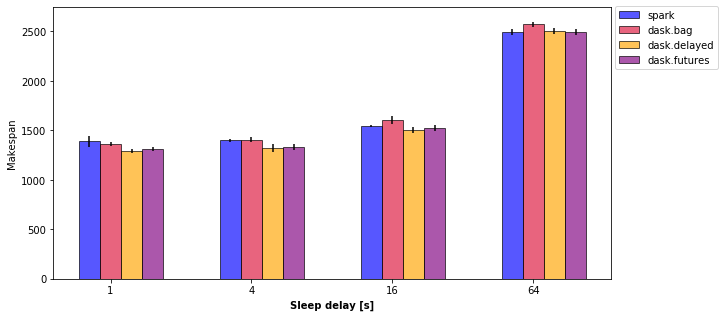
\includegraphics[clip,width=\columnwidth]{images/inc_sleep.png}%
    }
    
    \subfloat[Incrementation total time]{%
      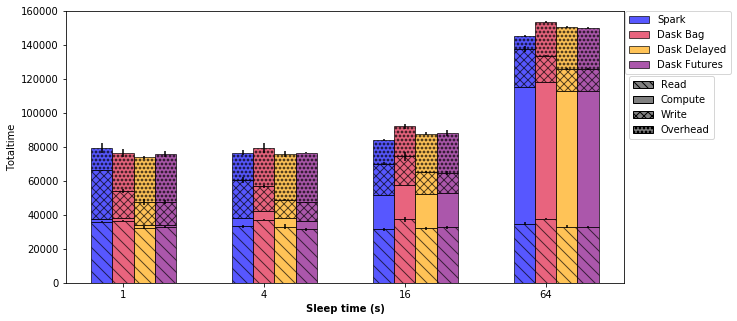
\includegraphics[clip,width=\columnwidth]{images/inc_idle_sleep.png}%
    }
    \caption{125 splits, 10 iterations, 8 instances}
    \label{fig:inc_sleep}
\end{figure}


% Chunks
\subsection{Experiment 1: Number of splits}
In Figure \ref{fig:inc_chunk} Spark is not compared for 30 chunks. This is because
spark has a 2GB limitation in the task size it can compute. Note from Figure
\ref{fig:inc_chunk}(b) that the compute time increase when there is more splits.
This is expected because the sleep delay is constant throughout this experiment and
there are more compute task when the number of splits increases. We also note that in
Figure \ref{fig:inc_chunk}(b) for 30 splits the dask bag api has a much lower
overhead time. This is because we only calculate the idle time of used core and the
dask bag api was only using one thread per block in comparison to the dask delayed
and dask futures api which were offloading the calculations on multiple thread of a
same worker. From Figure \ref{fig:inc_chunk} we observe that when the dataset is
seperated in more (smaller) splits it saves IO time however it increases the overhead
by a similar amount; the inverse happens when we reduce teh number of splits.

\begin{figure}[htp]
    \centering
    \subfloat[Incrementation makespan]{%
      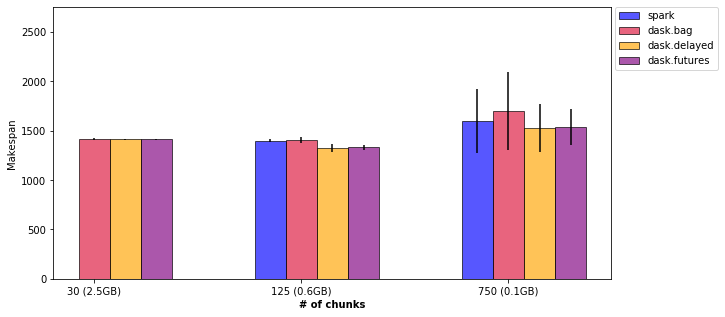
\includegraphics[clip,width=\columnwidth]{images/inc_chunk.png}%
    }
    
    \subfloat[Incrementation total time]{%
      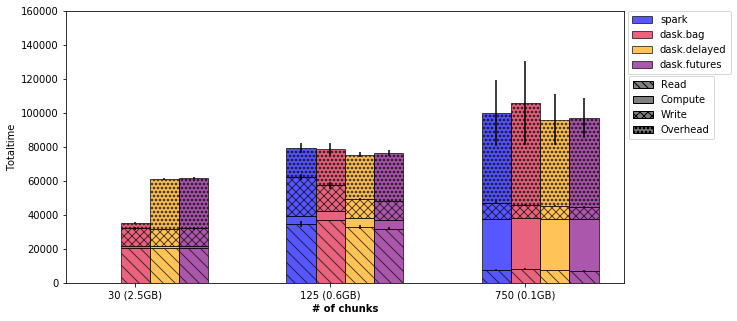
\includegraphics[clip,width=\columnwidth]{images/inc_idle_chunk.png}%
    }
    \caption{10 iterations, 4 sec. sleep delay, 8 instances}
    \label{fig:inc_chunk}
\end{figure}

From the Figures \ref{fig:inc_worker} to \ref{fig:inc_chunk} the Dask bag with optimized graph
has high variance on its makespan. Moreover, Dask API seems to always offer a better
option than spark RDDs.

%% Baseline gantt chart
\subsection{Experimentation 1: Baseline timeline}
From Table \ref{tb:inc-base} and Figure \ref{fig:inc_gantt} the framework have
similar makespan however the time spend for each type of task differ significantly.
Spark tends to spend more time than other framework for IO however it has a much
lower overhead. dask delayed and futures have a the loowest IO time but a much higher
overhead. Dask bag stand in the middle for both IO and overhead. Compute time is
approximately the same for all frameworks.

\begin{table}[h]
  \resizebox{\columnwidth}{!}{
    \begin{tabular}{|l|l|l|l|l|l|}
    \hline
    Framework    & Read     & Compute & Write    & Overhead & Total    \\ \hline
    Spark        & 34465.22 & 5117.90 & 22679.15 & 17075.94 & 79338.22 \\ \hline
    Dask.bag     & 36863.32 & 5120.80 & 15448.91 & 21387.82 & 78820.86 \\ \hline
    Dask.delayed & 32769.47 & 5119.32 & 11372.86 & 26198.90 & 75460.56 \\ \hline
    Dask.futures & 31891.29 & 5120.47 & 11269.66 & 27983.72 & 76265.14 \\ \hline
    \end{tabular}
  }
  \caption{Distirbution of the execution time in seconds}
  \label{tb:inc-base}
 \end{table}

\begin{figure}[htp]
    \centering
    \subfloat[Spark execution timeline]{%
      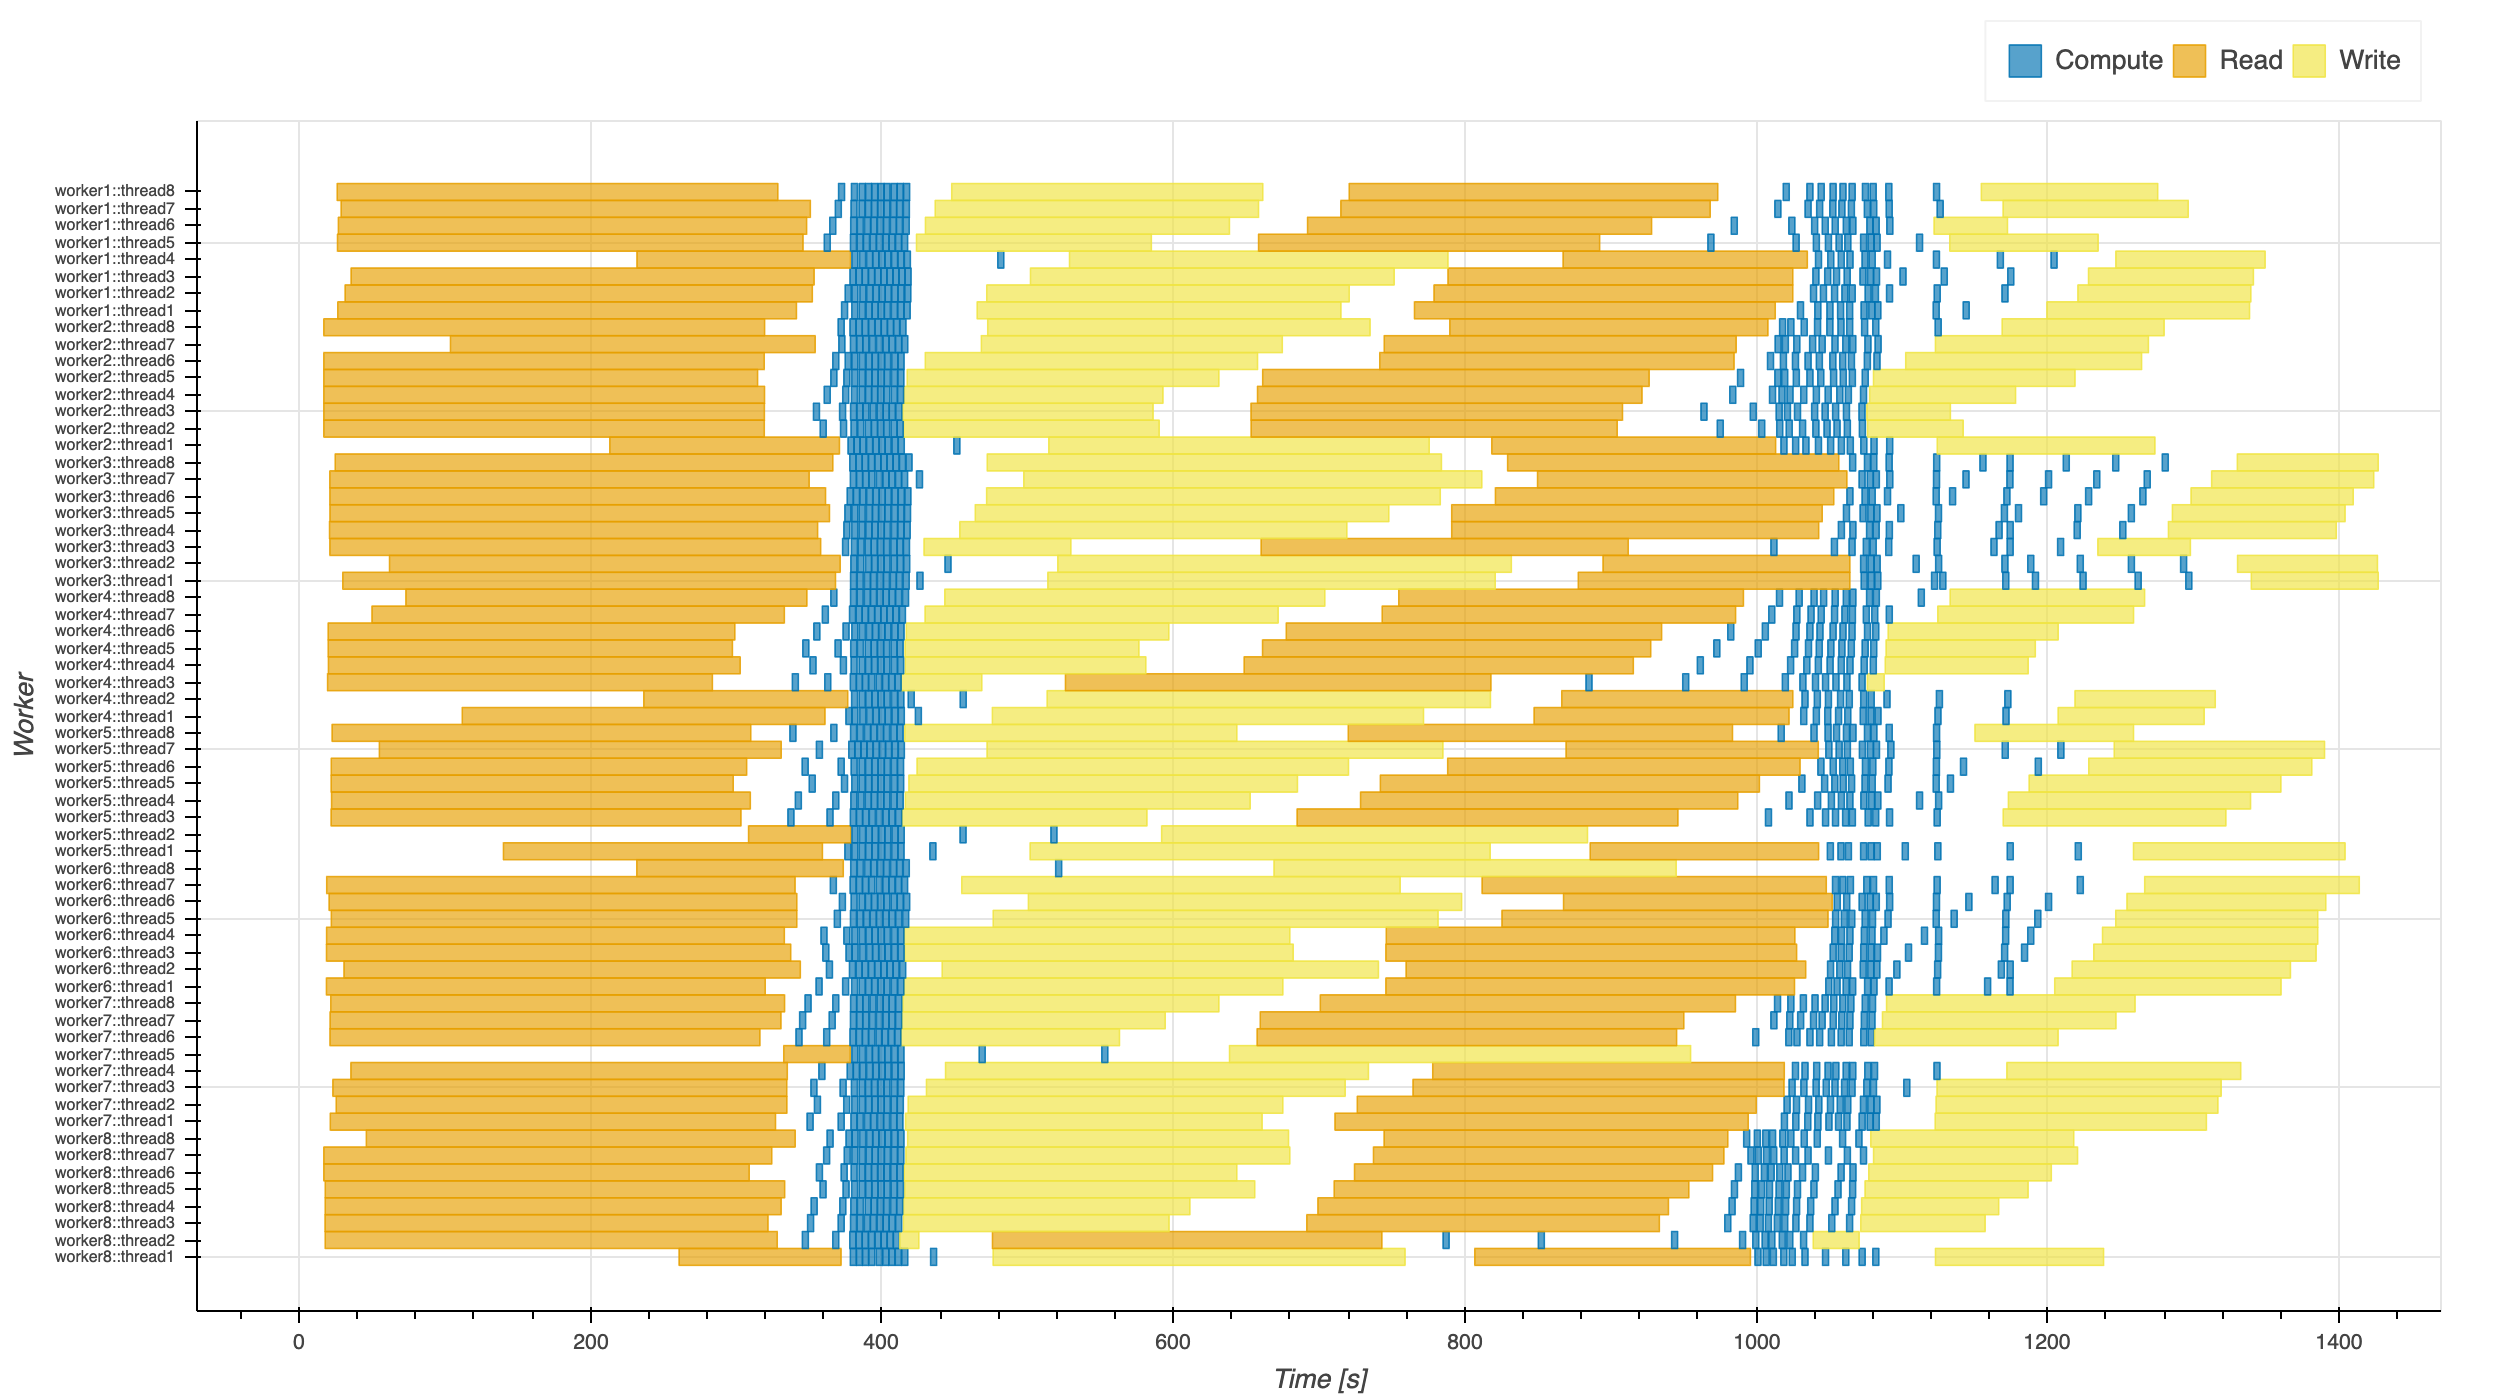
\includegraphics[clip,width=\columnwidth]{images/spark_inc_baseline_gantt.png}%
    }

    \subfloat[Dask bag execution timeline]{%
      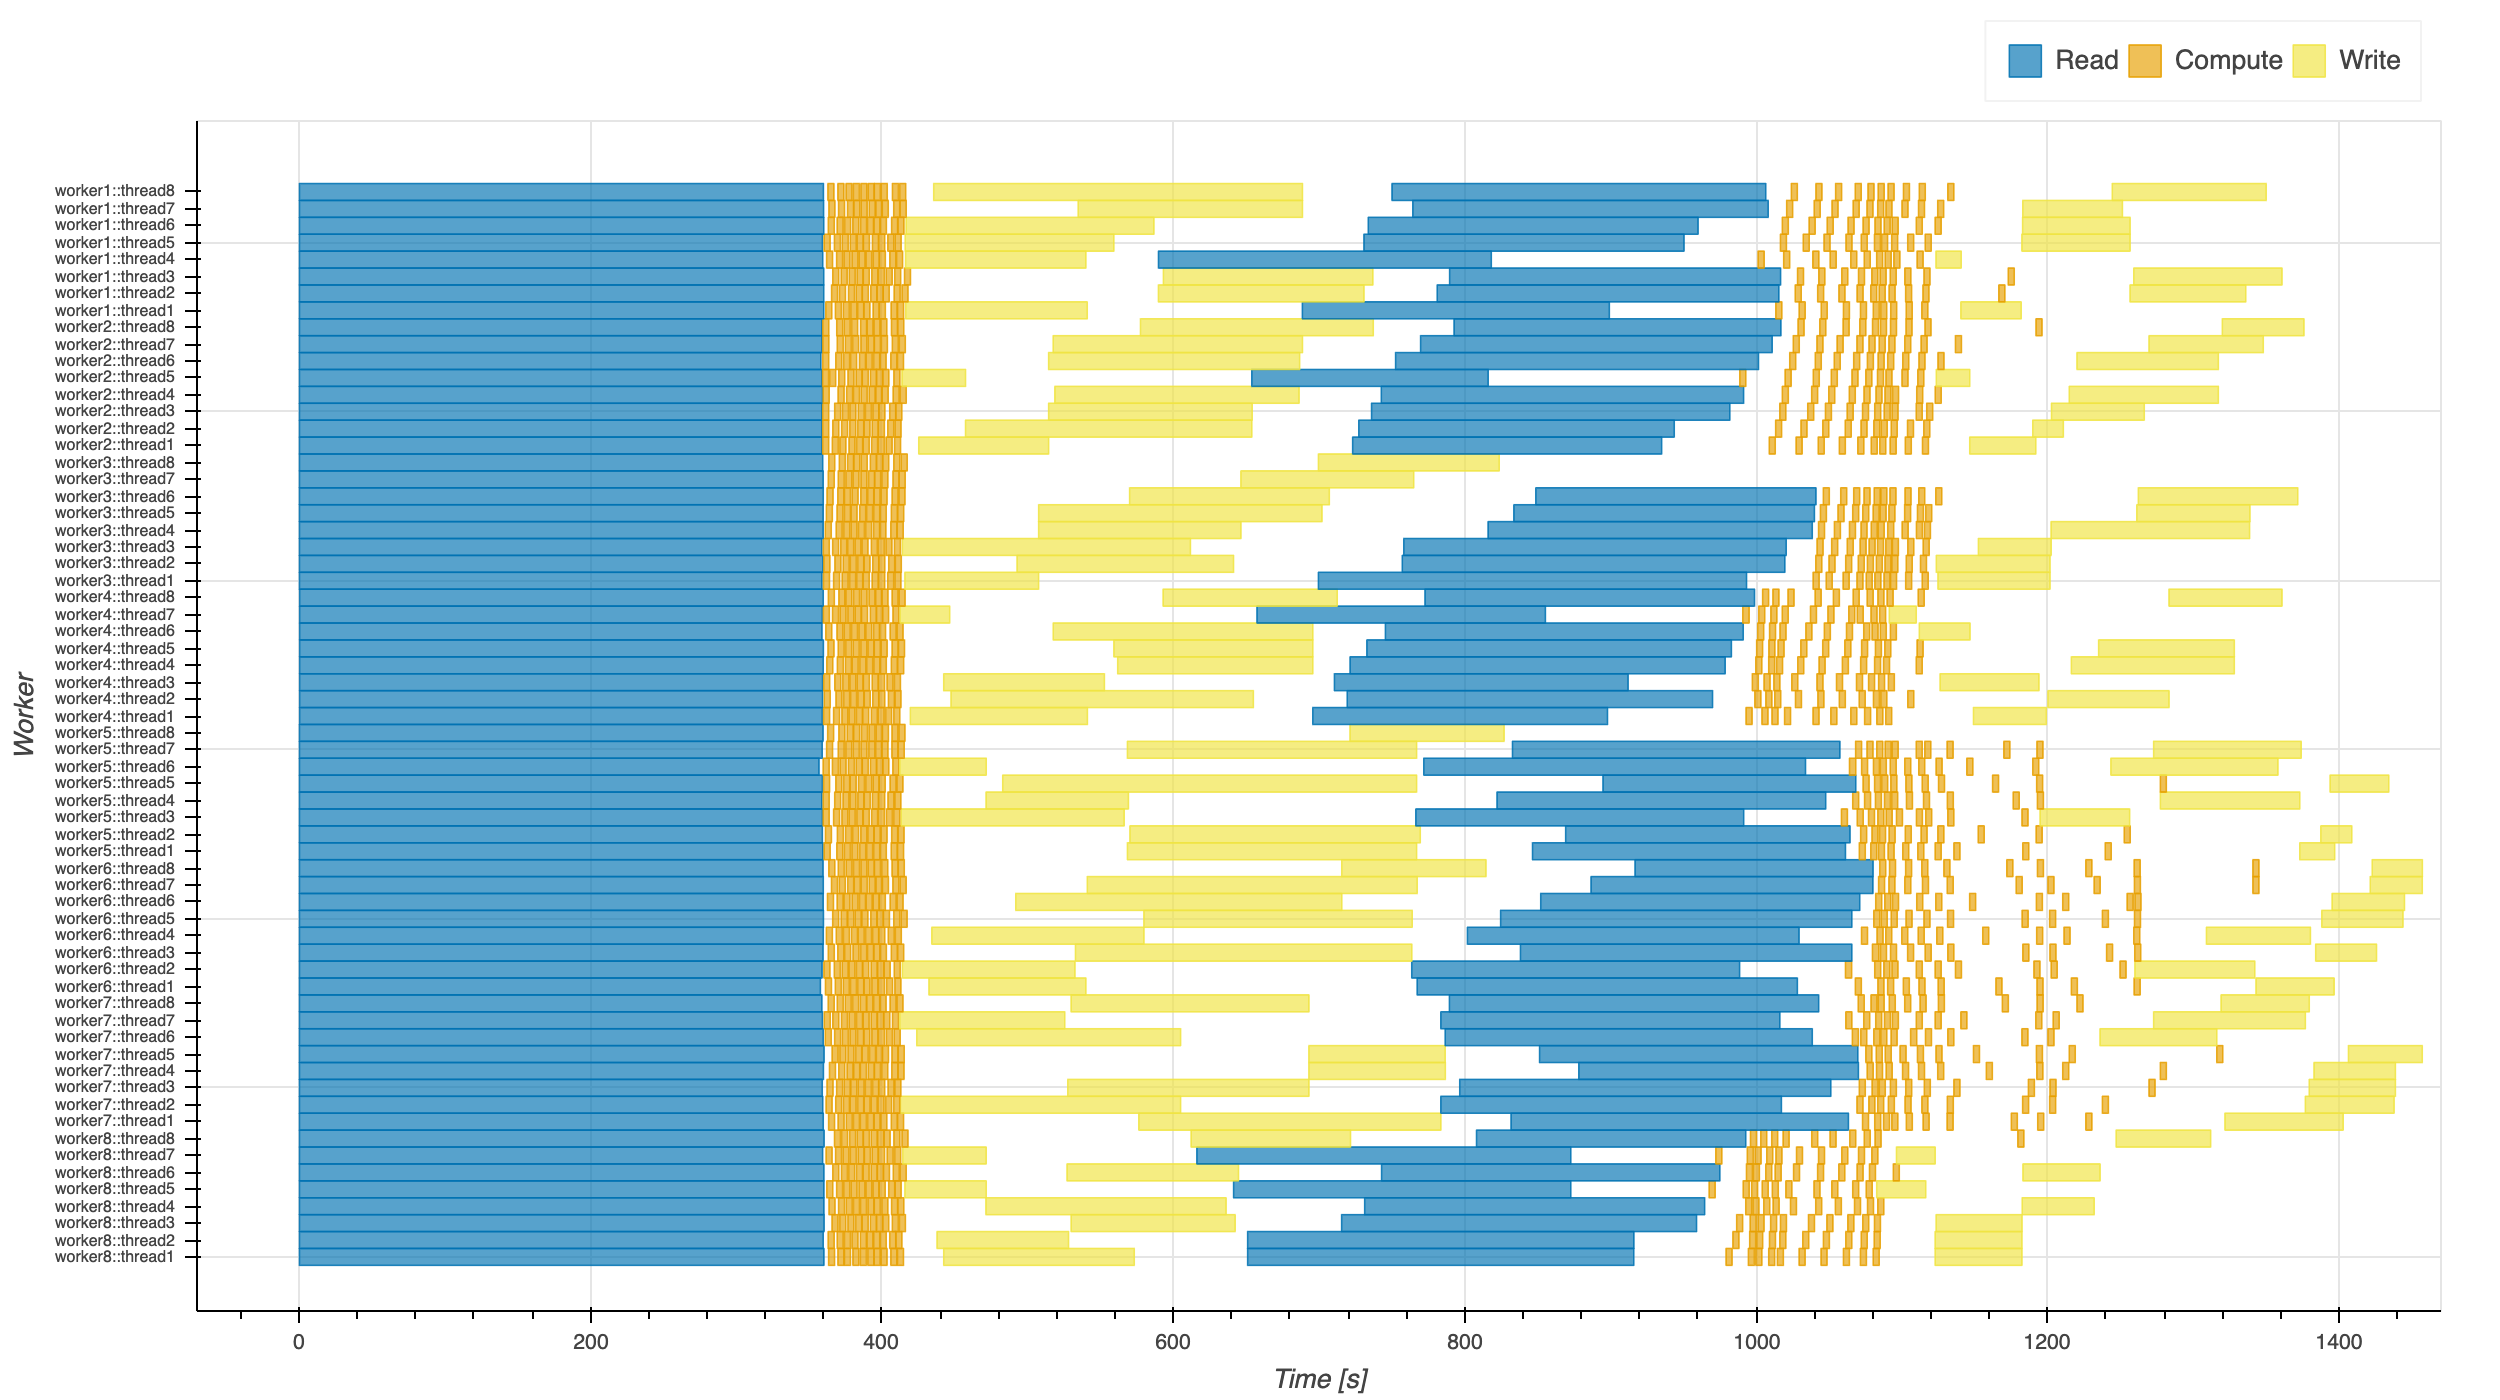
\includegraphics[clip,width=\columnwidth]{images/dask_bag_inc_baseline_gantt.png}%
    }

    \subfloat[Dask delayed execution timeline]{%
      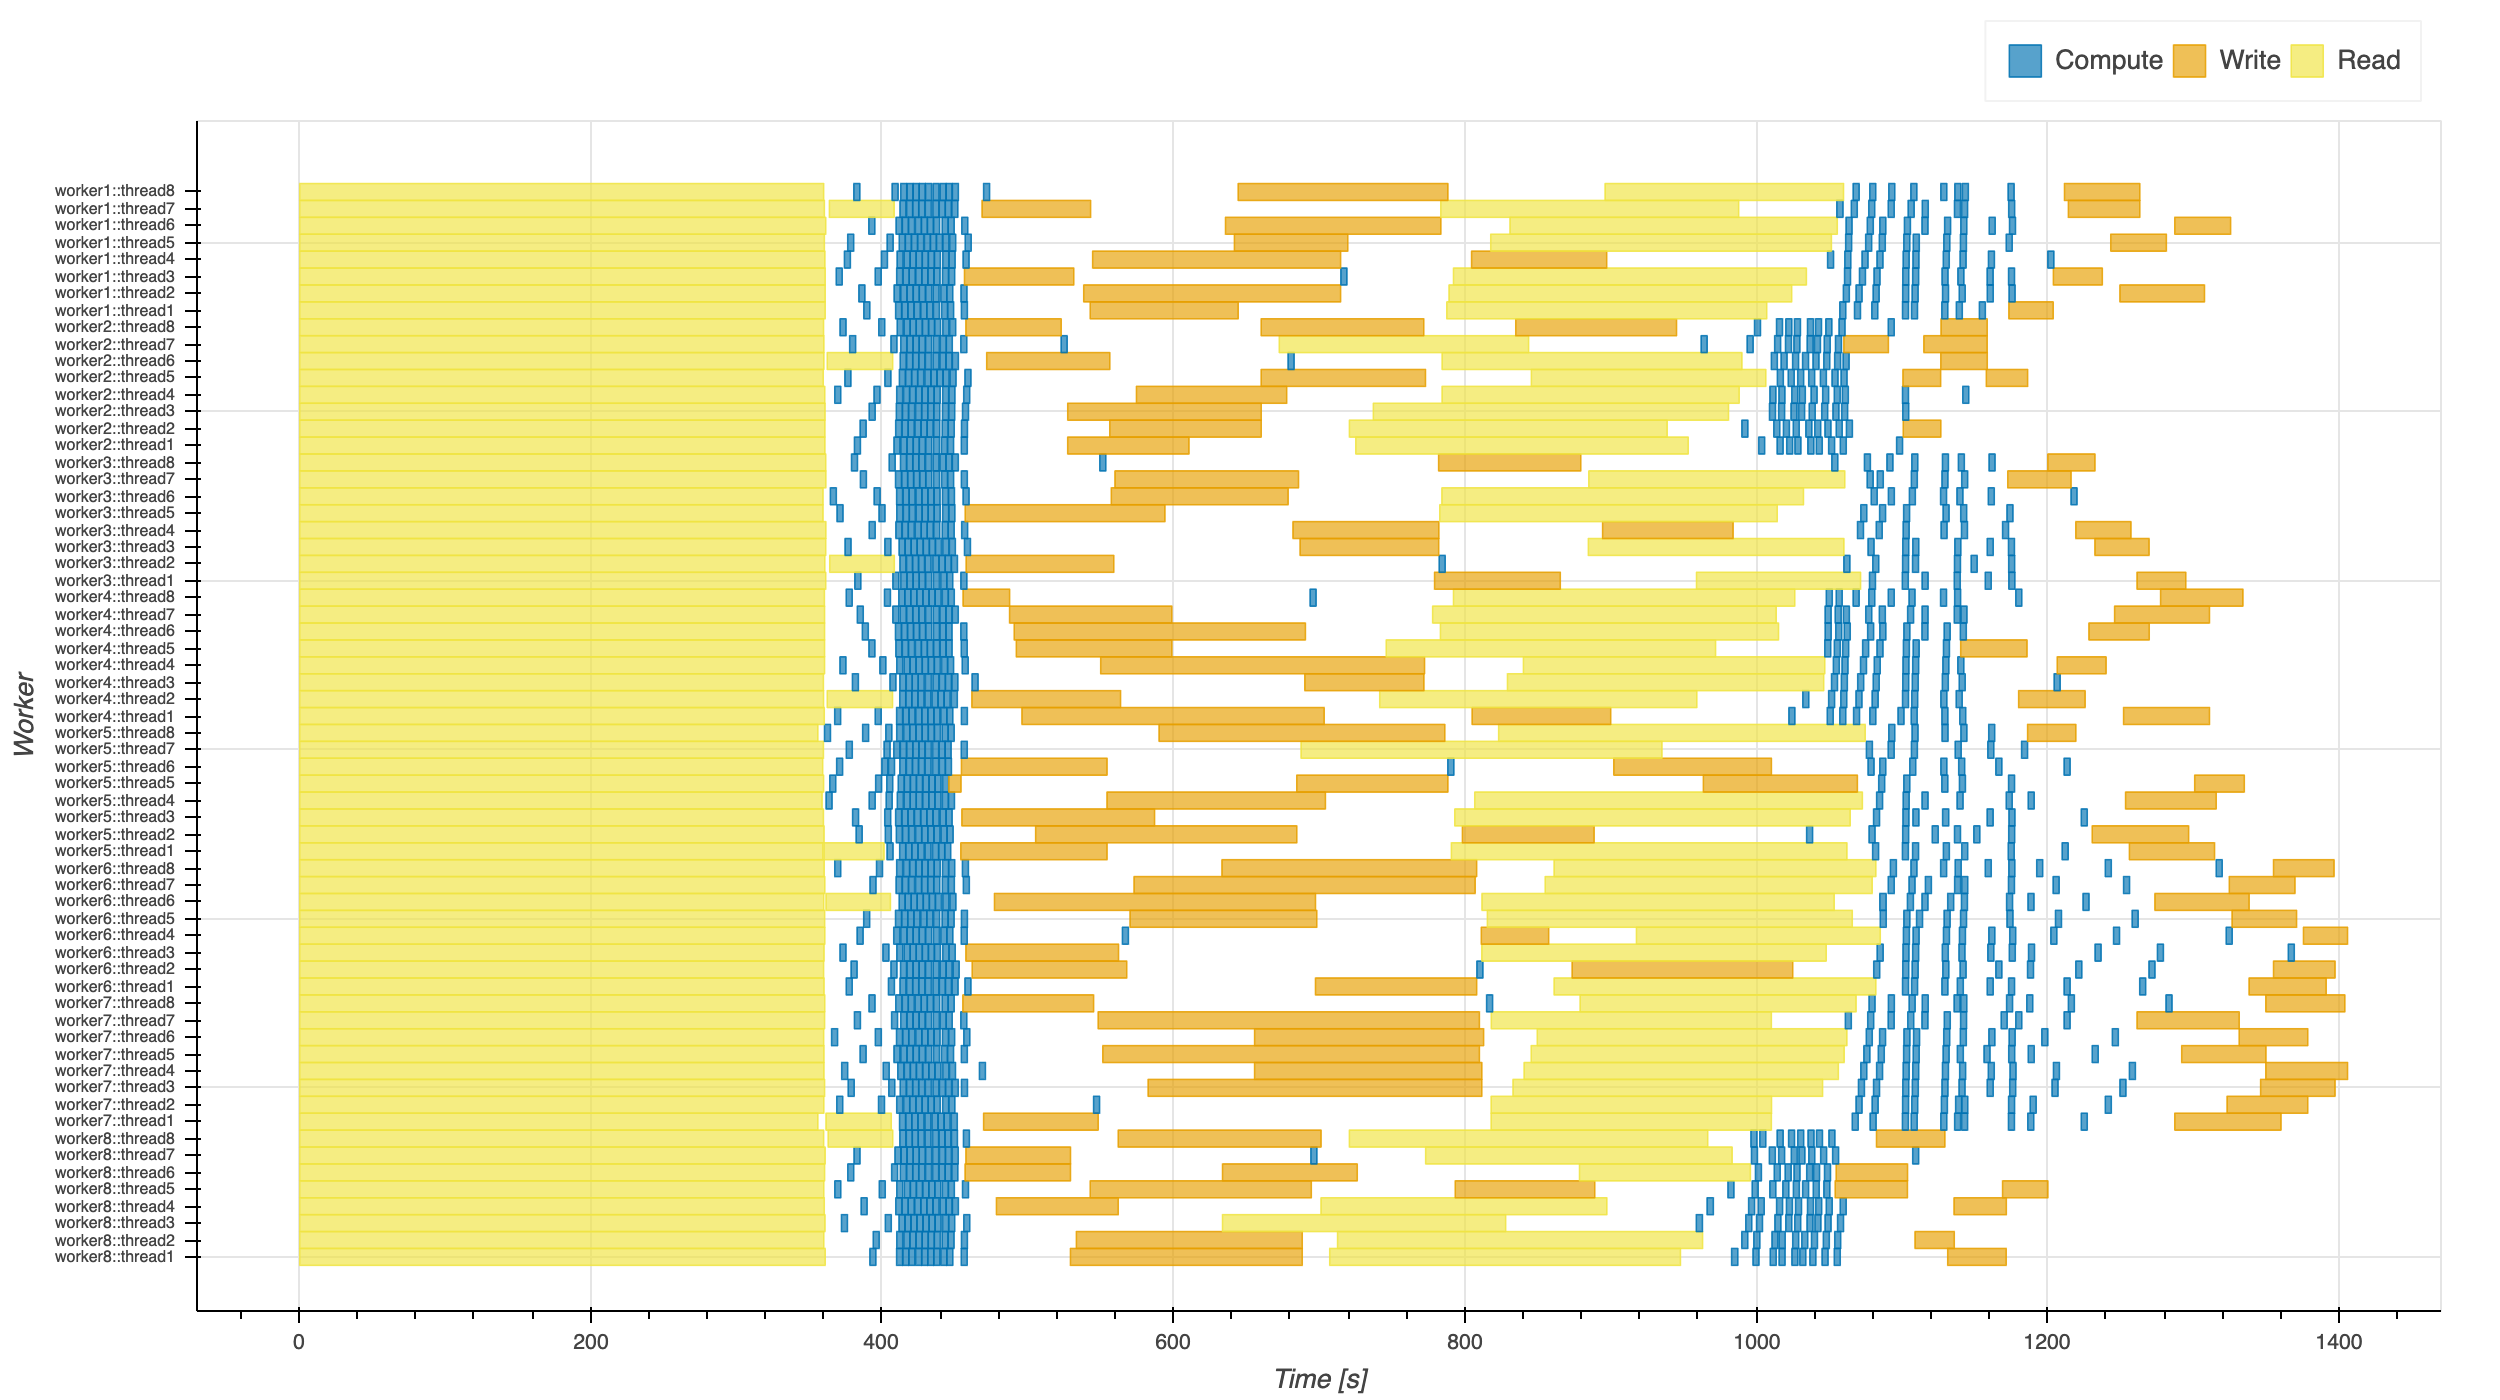
\includegraphics[clip,width=\columnwidth]{images/dask_delayed_inc_baseline_gantt.png}%
    }
    
    \subfloat[Dask futures execution timeline]{%
      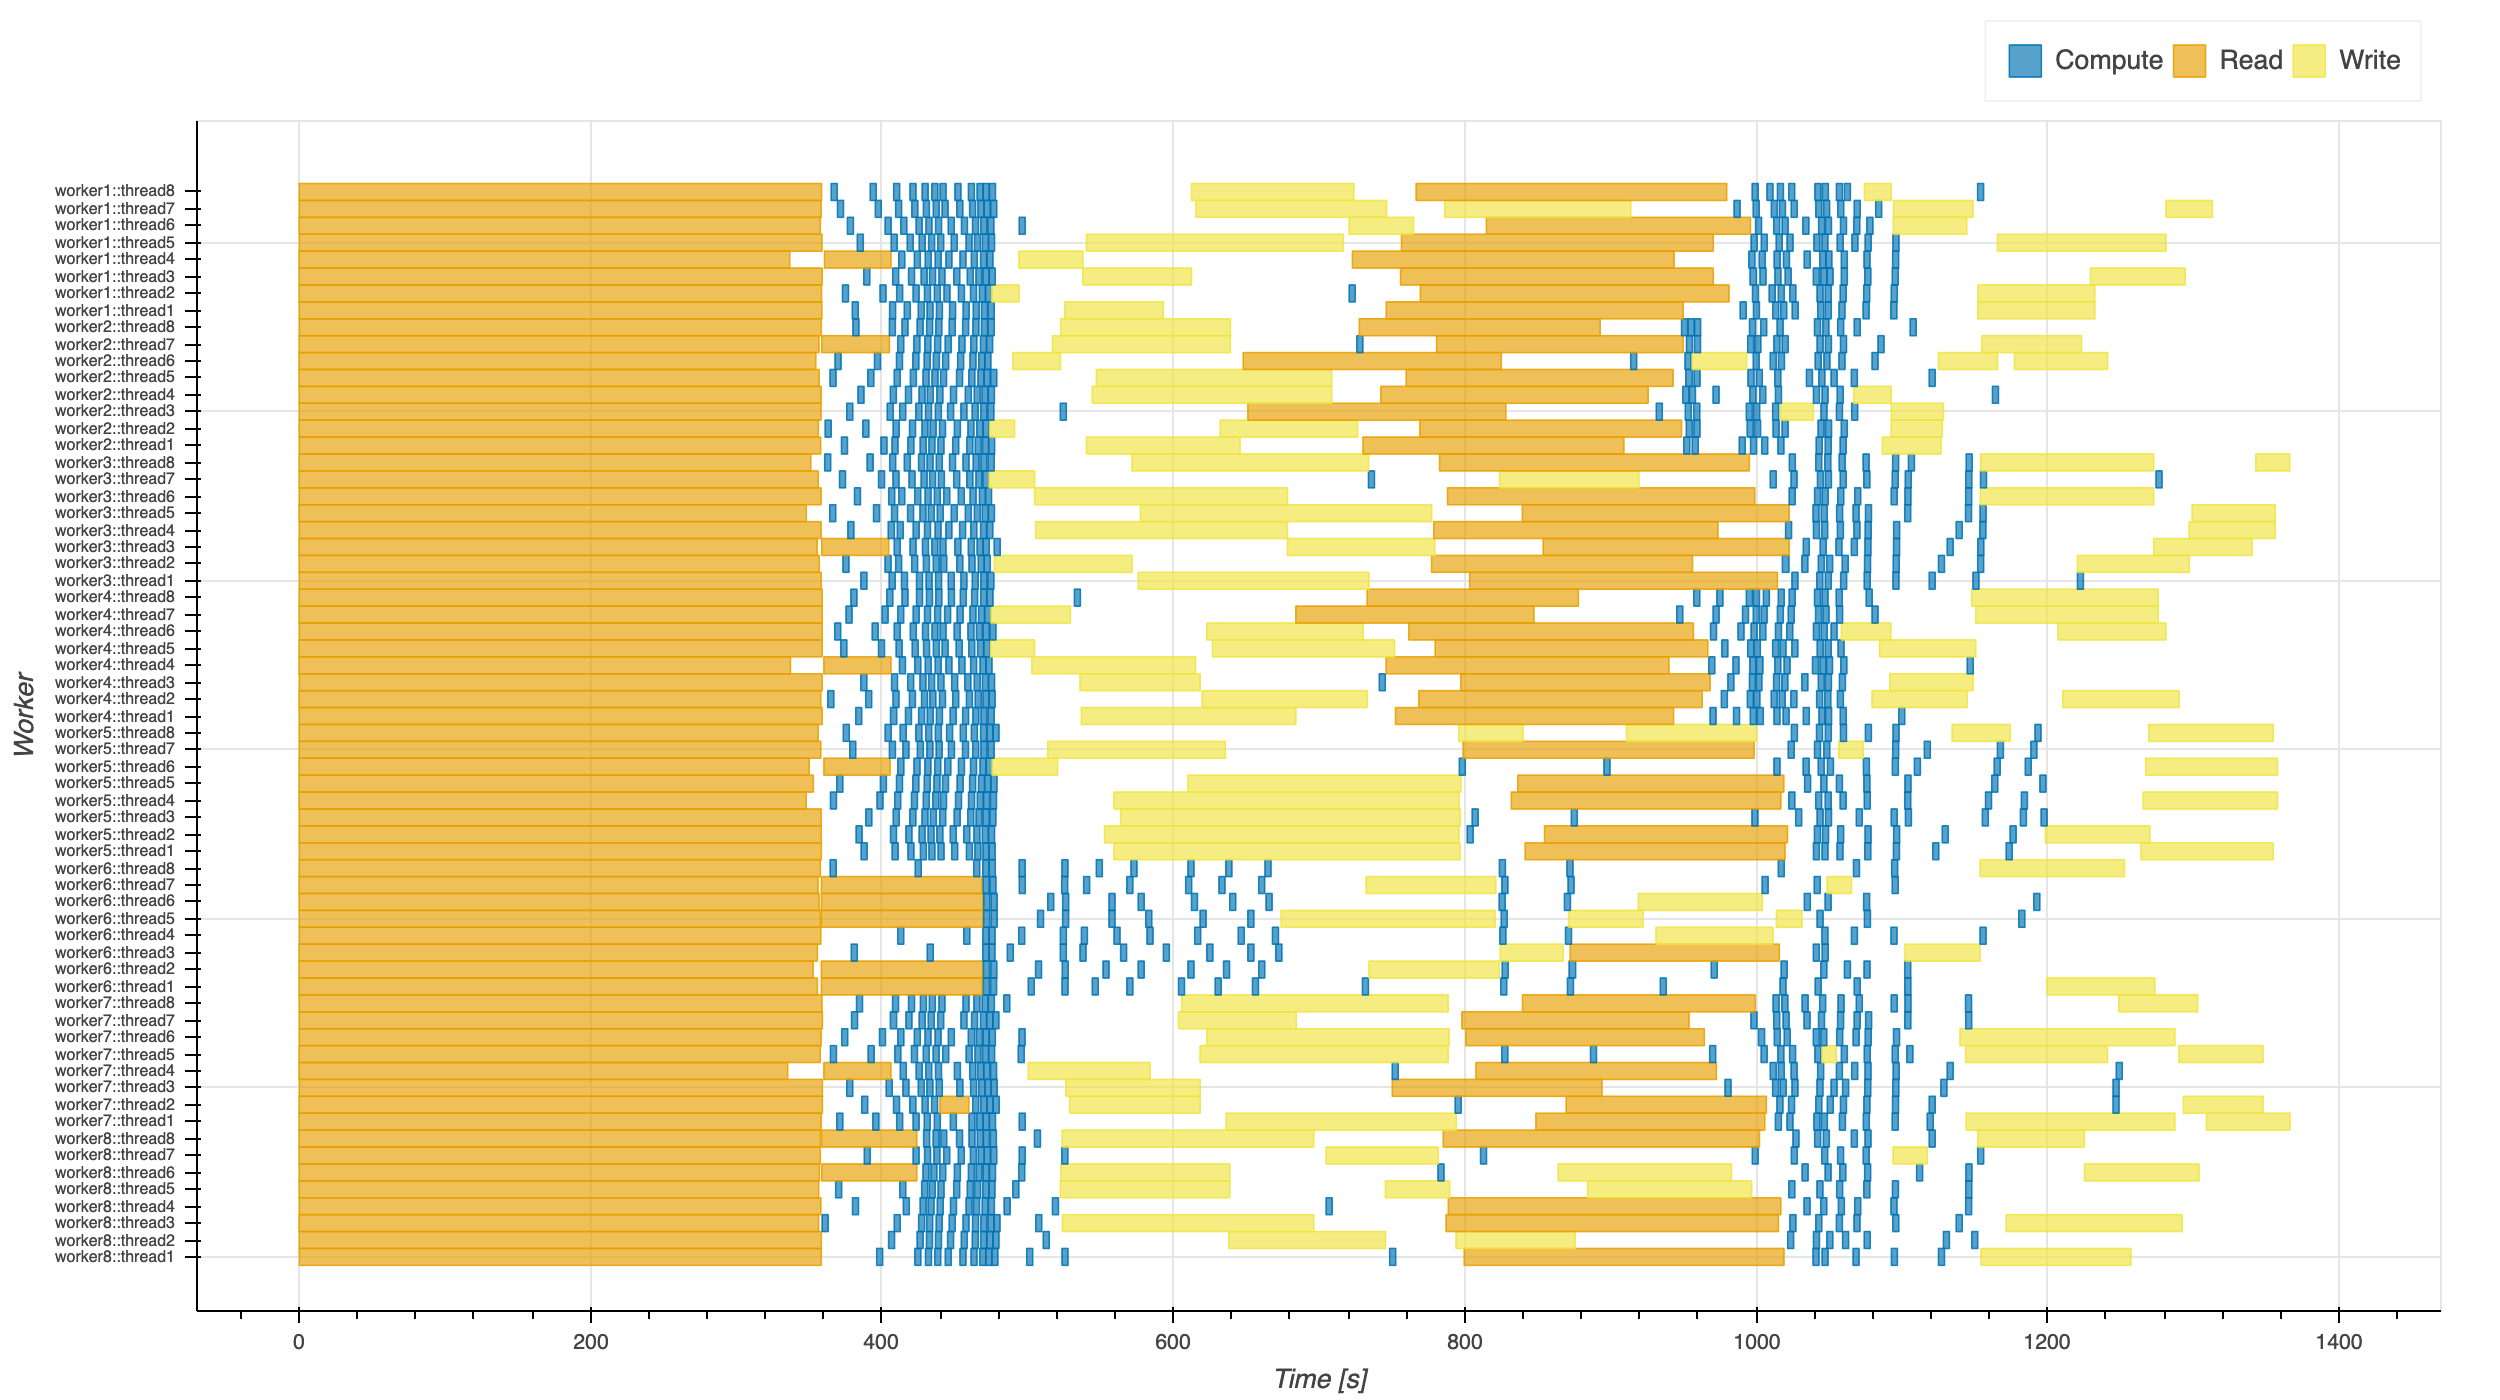
\includegraphics[clip,width=\columnwidth]{images/dask_futures_inc_baseline_gantt.png}%
    }
    \caption{125 splits, 4 sec. sleep delay, 8 instances}
    \label{fig:inc_gantt}
\end{figure}


%%% HISTOGRAM %%%
\subsection{Experiment 2: Number of instances}

\begin{figure}[htp]
    \centering
    \subfloat[Histogram makespan]{%
      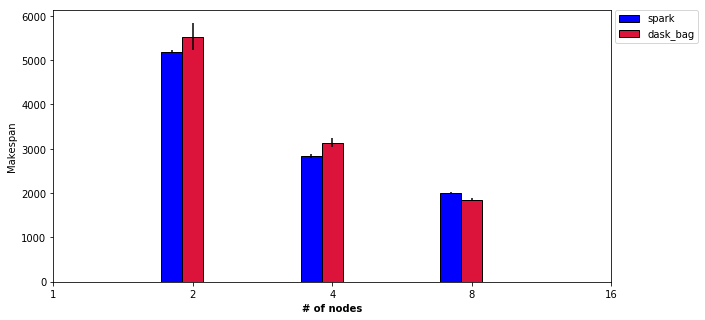
\includegraphics[clip,width=\columnwidth]{images/histo_instance.png}%
    }
    
    \subfloat[Histogram total time]{%
      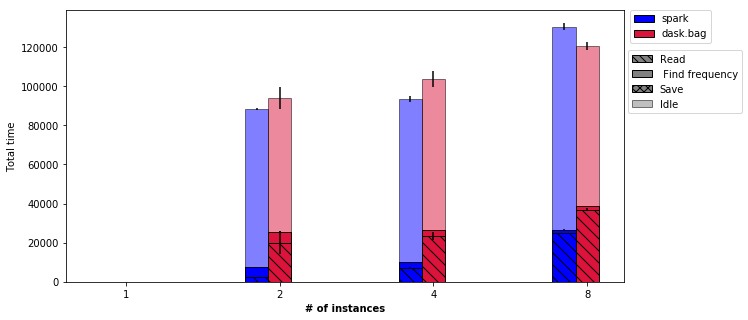
\includegraphics[clip,width=\columnwidth]{images/histo_idle_instances.png}%
    }
    \caption{8 instances}
    \label{fig:histo_wroker}
\end{figure}

\subsection{Experiment 2: Number of chunks}

\begin{figure}[htp]
    \centering
    \subfloat[Histogram makespan]{%
      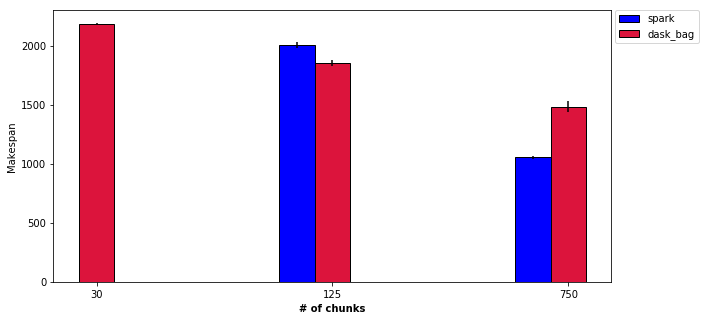
\includegraphics[clip,width=\columnwidth]{images/histo_splits.png}%
    }
    
    \subfloat[Histogram total time]{%
      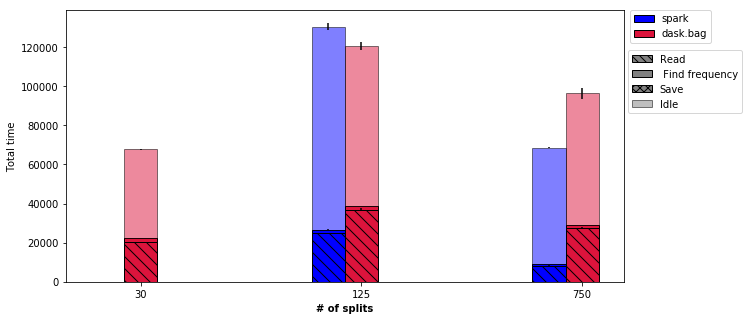
\includegraphics[clip,width=\columnwidth]{images/histo_idle_splits.png}%
    }
    \caption{10 iterations, 4 sec. sleep delay, 8 instances}
    \label{fig:histo_chunk}
\end{figure}

%%% BIDS EXAMPLE %%%
\subsection{Experiment 3: Number of instances}



%%%%% DISCUSSION %%%%%
\section{Discussion}
\subsection{IO Time}


\subsection{Serialization}
We think that serialization could have an important effect on the makespan of the
application. This could potentially slow down the application when a lot of tasks are
scheduled.

\subsection{NFS}
The nfs seems to be a source of bottleneck. We think that exploring other file
system, like Lustre, could give us insight the actual effect of the nfs on the
application makespan. We also think that the nfs caching could play an effect on the
task of different length.

\subsection{Scheduler}
The Dask scheduler seems to have some bizarre behaviour. It seems like it waits to
schedule task. However it could also be due to tasks being scheduled on other workers
thus requiring data to be sent over the network; which would explain the stall on the
worker. More work would be needed to investigate that issue.


\subsection{Caching}
We think that caching plays an effect on the results. As seen in the gantt chart
previously, some of the read tasks are significantly shorter than other while all
chunks are of equal size.



%% Future work
\subsection{Future work}
There is definitely a lot of work to be done to assess exactly what is happening at
the scheduling level for both Dask and Spark. For the future we plan to test the
effect of caching on the system. We would also need to explore caching and saturation
of the nfs. We also need to explore different scheduler (e.g. Yarn, Mesos) on both
Spark and Dask to see if our result are mostly affected by the scheduler or outside
factors. Afterwards, we want to continue the analysis by evaluating the memory
consumption of the frameworks. Moreover we want to explore more complex algorithm
including some related to neuroimaging. We also plan to investigate which library
would be better in which context.

\section{Acknowledgement}
We would like to thanks Compute Canada Cloud for the the infrastructure.

\bibliography{acl2019}
\bibliographystyle{acl_natbib}

\end{document}
